\section{Appendix A: Proofs}
\label{proofs-general}

\subsection{Proofs of the results in section~\ref{general}}

Let us now consider the establishment of the convergence theory given in section~\ref{general}.

{\bf Proof of Lemma 1.}
Let $\rho(t)=f(w^r+td^r)$ and $\gamma(t)=\rho(t)-\rho(0)-\alpha t\rho^\prime(0)$.
Note the following connections with quantities involved in Lemma 1: $\rho(t)=f^{r+1}$, $\rho(0)=f^r$, $\rho^\prime(t)=g^{r+1}\cdot d^r$ and $\gamma(t)=f^{r+1} - f^r - \alpha g^r\cdot(w^{r+1}-w^r)$.
(\ref{ag}) corresponds to the condition $\gamma(t)\le 0$ and (\ref{wolfe}) corresponds to the condition $\rho^\prime(t)\ge \beta\rho^\prime(0)$.

$\gamma^\prime(t) = \rho^\prime(t)-\alpha \rho^\prime(0)$.
$\rho^\prime(0)<0$.
$\rho^\prime$ is strictly monotone increasing because, by assumption A2,
\begin{equation}
\rho^\prime(t)-\rho^\prime(\ttilde) \ge \sigma (t-\ttilde)\|d^r\|^2 \;\; \forall \; t, \ttilde
\label{prop11}
\end{equation}
This implies that $\gamma^\prime$ is also strictly monotone increasing and, all four, $\rho$, $\rho^\prime$, $\gamma^\prime$ and $\gamma$ tend to infinity as $t$ tends to infinity.

Let $t_\beta$ be the point at which $\rho^\prime(t)=\beta\rho^\prime(0)$. Since $\rho^\prime(0)<0$ and $\rho^\prime$ is strictly monotone increasing, $t_\beta$ is unique and $t_\beta>0$. This validates the definition in (\ref{tbeta}). Monotonicity of $\rho^\prime$ implies that (\ref{wolfe}) is satisfied iff $t\ge t_\beta$.

Note that $\gamma(0)=0$ and $\gamma^\prime(0)<0$. Also, since $\gamma^\prime$ is monotone increasing and $\gamma(t)\to\infty$ as $t\to\infty$, there exists a unique $t_\alpha>0$ such that $\gamma(t_\alpha)=0$, which validates the definition in (\ref{talpha}). It is easily checked that $\gamma(t)\le 0$ iff $t\in [0,t_\alpha]$.

The properties also imply $\gamma^\prime(t_\alpha)> 0$, which means $\rho^\prime(t_\alpha) \ge \alpha\rho^\prime(0)$. By the monotonicity of $\rho^\prime$ we get $t_\alpha>t_\beta$, proving the lemma.


{\bf Proof of Theorem 2.} Using (\ref{wolfe}) and A1,
\begin{equation}
(\beta-1)g^r\cdot d^r \le (g^{r+1}-g^r)\cdot d^r \le Lt\|d^r\|^2
\label{th21}
\end{equation}
This gives a lower bound on $t$:
\begin{equation}
t \ge \frac{(1-\beta)}{L\|d^r\|^2} (-g^r\cdot d^r)
\label{th22}
\end{equation}
Using (\ref{ag}), (\ref{th22}) and (\ref{angle}) we get
\begin{eqnarray}
f^{r+1} & \le & f^r + \alpha t g^r\cdot d^r \nonumber \\
        & \le & f^r - \frac{\alpha(1-\beta)}{L\|d^r\|^2} (-g^r\cdot d^r)^2 \nonumber \\
        & \le & f^r - \frac{\alpha(1-\beta)}{L} \cos^2 \theta \|g^r\|^2
\label{th23}
\end{eqnarray}
Subtracting $f^\star$ gives
\begin{equation}
(f^{r+1} - f^\star) \le  (f^r-f^\star) - \frac{\alpha(1-\beta)}{L} \cos^2 \theta \|g^r\|^2
\label{th24}
\end{equation}
A2 together with $g(w^\star)=0$ implies $\|g^r\|^2\ge\sigma^2\|w^r-w^\star\|^2$. Also A1 implies $f^r-f^\star \le \frac{L}{2}\|w^r-w^\star\|^2$~\cite{smola2008}. Using these in (\ref{th24}) gives
\begin{eqnarray}
(f^{r+1}-f^\star) & \le & (f^r - f^\star) - 2\alpha(1-\beta)\frac{\sigma^2}{L^2} \cos^2\theta (f^r - f^\star) \nonumber \\
                  & \le & (1 - 2\alpha(1-\beta)\frac{\sigma^2}{L^2} \cos^2\theta) (f^r - f^\star)
\label{th25}
\end{eqnarray}
Let $\delta = (1 - 2\alpha(1-\beta)\frac{\sigma^2}{L^2} \cos^2\theta)$. Clearly $0 < \delta < 1$. Theorem 2 follows.

\subsection{Proofs of the results in section~\ref{distr}}

Let us now consider the establishment of the convergence theory given in section~\ref{distr}. We begin by establishing that the exact minimizer of $\fhat_p$ makes a sufficient angle of descent at $w^r$.

{\bf Lemma 5.} Let $\what_p^\star$ be the minimizer of $\fhat_p$. Let $d_p= (\what_p^\star-w^r)$. Then
\begin{equation}
-g^r\cdot d_p \ge (\sigma/L) \|g^r\| \|d_p\|
\label{suffangle}
\end{equation}

{\bf Proof.} First note, using gradient consistency and $\grad f_p(\what_p^\star)=0$ that
\begin{equation}
\|g^r\| = \| \grad \fhat_p(w^r)-\grad \fhat_p(\what_p^\star) \| \le L\|d_p\|
\label{lem211}
\end{equation}
Now,
\begin{eqnarray}
-g^r\cdot d_p &=&(\grad \fhat_p(w^r)-\grad \fhat_p(\what_p^\star))^T(w^r-\what_p^\star) \nonumber \\
            &\ge& \sigma \|d_p\|^2 \nonumber \\
            &=& \sigma \|g^r\| \|d_p\| \frac{\|d_p\|}{\|g^r\|} \nonumber \\
            &\ge& \frac{\sigma}{L} \|g^r\| \|d_p\|
\label{lem212}
\end{eqnarray}
where the second line comes from $\sigma$-strong convexity and the fourth line follows from (\ref{lem211}).

{\bf Proof of Lemma 3.}
Let us now turn to the question of approximate stopping and establish Lemma 3. Given $\theta$ satisfying (\ref{thetadef}) let us choose $\zeta\in (0,1)$ such that
\begin{equation}
\label{lem2211}
\frac{\pi}{2} > \theta > \cos^{-1} \frac{\sigma}{L} + \cos^{-1} \zeta
\end{equation}

%{\bf Lemma 7.} Assume $g(w^r)\not=0$. Suppose we minimize $\fhat_p$ using an optimizer that starts from $v^0=w^r$ and generates a sequence $\{v^k\}$ having linear convergence, i.e.,
%\begin{equation}
%\fhat_p(v^{k+1}) - \fhat_p^\star \le \delta (\fhat_p(v^k) - \fhat_p^\star)
%\label{22a}
%\end{equation}
%where $\fhat_p^\star = \fhat_p(\what_p^\star)$. Then, given any $\zeta$ satisfying $0<\zeta<1$, there exists $\khat$ (which depends only on $\zeta$, $\sigma$ and $L$) such that
%\begin{equation}
%\cos \phi^k \ge \zeta \;\; \forall k\ge \khat
%\label{22b}
%\end{equation}
%where $\phi^k$ is the angle between $\what_p^\star-w^r$ and $v^k-w^r$.

%fhat to fhat_p

%Add a diagram to help
\begin{figure}
\begin{center}
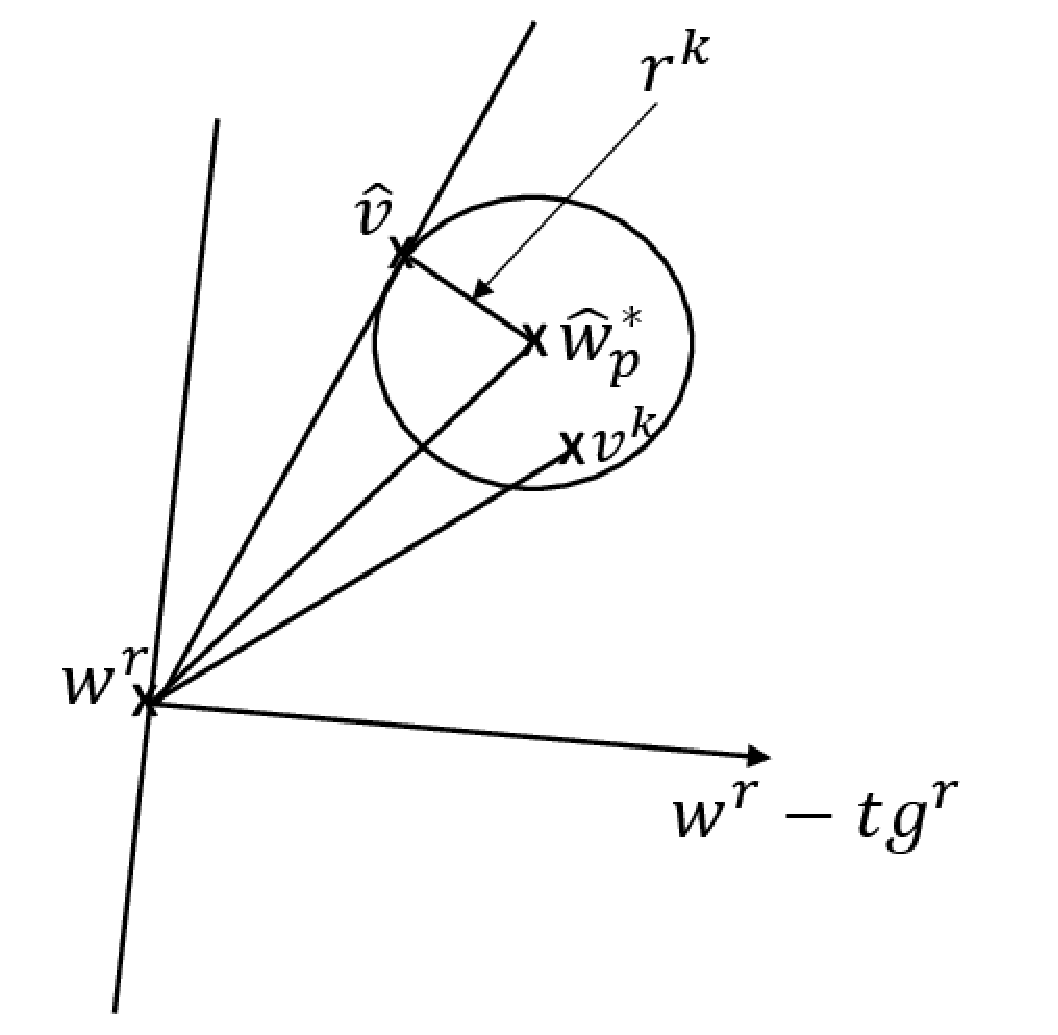
\includegraphics[width=0.8\columnwidth]{figures/spherefig}
\caption{Construction used in the proof of Lemma 3.}
\end{center}
\label{spherefig}
\end{figure}


By A3 and equations ($3.16$) and ($3.22$) in~\cite{smola2008}, we get
\begin{equation}
\frac{\sigma}{2} \|v-\what_p^\star\|^2 \le \fhat_p(v) - \fhat_p^\star \le \frac{L}{2} \|v-\what_p^\star\|^2
\label{lem221}
\end{equation}
After $k$ iterations we have
\begin{equation}
\fhat_p(v^k) - \fhat_p^\star \le \delta^k (\fhat_p(w^r) - \fhat_p^\star)
\label{lem222}
\end{equation}
We can use these to get
\begin{eqnarray}
\|v^k-\what_p^\star\|^2 &\le& \frac{2(\fhat_p(v^k)-\fhat_p^\star)}{\sigma} \nonumber \\
                        &\le& \frac{2\delta^k (\fhat_p(w^r)-\fhat_p^\star)}{\sigma} \nonumber \\
                        &\le& \frac{\delta^kL}{\sigma} \|w^r-\what_p^\star\|^2 \defs (r^k)^2
\label{lem223}
\end{eqnarray}
For now let us assume the following:
\begin{equation}
\|v^k-\what_p^\star\|^2 \le \|w^r-\what_p^\star\|^2
\label{lem224}
\end{equation}
Using (\ref{lem223}) note that (\ref{lem224}) holds if
\begin{equation}
\frac{\delta^kL}{\sigma} \le 1
\label{lem225}
\end{equation}
Let $S^k$ be the sphere, $S^k = \{ v : \|v-\what_p^\star\|^2 \le (r^k)^2 \}$. By (\ref{lem223})
%and (\ref{lem224})
we have $v^k\in S^k$. See Figure~\ref{spherefig}. Therefore,
\begin{equation}
\phi^k \le \max_{v\in S^k} \phi(v)
\label{lem226}
\end{equation}
where $\phi^k$ is the angle between $\what_p^\star-w^r$ and $v^k-w^r$, and $\phi(v)$ is the angle between $v-w^r$ and $\what_p^\star-w^r$. Given the simple geometry, it is easy to see that $\max_{v\in S^k} \phi(v)$ is attained by a point $\vhat$ lying on the boundary of $S^k$ (i.e., $\|\vhat-\what_p^\star\|^2 = (r^k)^2$) and satisfying $(\vhat-\what_p^\star)\perp (\vhat-w^r)$. This geometry yields
\begin{eqnarray}
\cos^2 \phi(\vhat) &=& \frac{\|\vhat-w^r\|^2}{\|\what_p^\star-w^r\|^2} \nonumber \\
                   &=& \frac{\|\what_p^\star-w^r\|^2-(r^k)^2}{\|\what_p^\star-w^r\|^2} \nonumber \\
                   &=& 1-\frac{(r^k)^2}{\|\what_p^\star-w^r\|^2} = 1-\frac{\delta^kL}{\sigma}
\label{lem227}
\end{eqnarray}
Since $\phi^k\le \phi(\vhat)$,
\begin{equation}
\cos^2 \phi^k \ge 1-\frac{\delta^kL}{\sigma}
\label{lem228}
\end{equation}
Thus, if
\begin{equation}
1-\frac{\delta^kL}{\sigma} \ge \zeta^2
\label{lem229}
\end{equation}
then
\begin{equation}
\cos \phi^k \ge \zeta \;\; \forall k\ge \khat
\label{22b}
\end{equation}
holds. By (\ref{lem2211}) this yields $\phase{-g^r,v^k-w^r} \le \theta$, the result needed in Lemma 3. Since $\zeta>0$, (\ref{lem229}) implies (\ref{lem225}), so (\ref{lem224}) holds and there is no need to separately satisfy it. Now (\ref{lem229}) holds if
\begin{equation}
k \ge \khat \defs \frac{\log (L/(\sigma(1-\zeta^2)))}{\log(1/\delta)}
\label{lem2210}
\end{equation}
which proves the lemma.

{\bf Proof of Theorem 4.} It trivially follows from a combination of Lemma 3 and Theorem 2.

